\documentclass{beamer}
\usepackage[utf8]{inputenc}
\usepackage{dsfont}
\usetheme{Darmstadt}
\usecolortheme{default}

\begin{document}



%---
%This block of code defines the information to appear in the Title page
\title[About Beamer]{Does Urbanisation Predict Election Outcomes?}

\subtitle{A Bayesian's Perspective}

\author[Odole, Cunha, Murthy] % (optional)
{Eldaleona ~Odole \and Leonor ~Cunha \and Anarghya ~Murthy }

\institute[Technische Universität Dortmund] % (optional)
{
  
  Faculty of Statistics\\
}

\date{\today} % (optional)
% {Mid-Term Presentation}

\logo{
\includegraphics[height=0.5cm]{tu.pdf}}

%End of title page configuration block
%---

%---
%The next block of commands puts the table of contents at the beginning of each section and highlights the current section:
% \AtBeginSection[]
% {
%   \begin{frame}
%     \frametitle{Table of Contents}
%     \tableofcontents[currentsection]
%   \end{frame}
% }
%---



%The next statement creates the title page.
\frame{\titlepage}

%---
%This block of code is for the table of contents after
%the title page
\begin{frame}
\frametitle{Table of Contents}
\tableofcontents
\end{frame}
%---

%---SECTION 1: INTRO
\section{Introduction}

\begin{frame}
\frametitle{Introduction}
\begin{itemize}
  \item \textbf{Research Question:}
  How does urbanization of a particular district affect result of an election in the US? 
  \item \textbf{Variable of Interest:}
  Winning party in the  House of Representatives 2022 General Election (binary)
\end{itemize}
\end{frame}



%slide
\section{Dataset Description}
\begin{frame}
\frametitle{Dataset}
We wanted to consider different factors in the analysis, with our primary focus being the urbanization of each House district. These factors included: 
\begin{enumerate}
  \item Demographic Data (US Census Bureau)
  \item Urbanization (FiveThirtyEight)
  \item Regional Information (US Census Bureau)
  \item Election Results (FiveThirtyEight)
\end{enumerate}
We combined different sources in order to create our data set containing 435 instances of 16 unique covariates.
\end{frame}  


\begin{frame}{Winning Party}
Our independent variable is Winning party in the 2022 Election.
 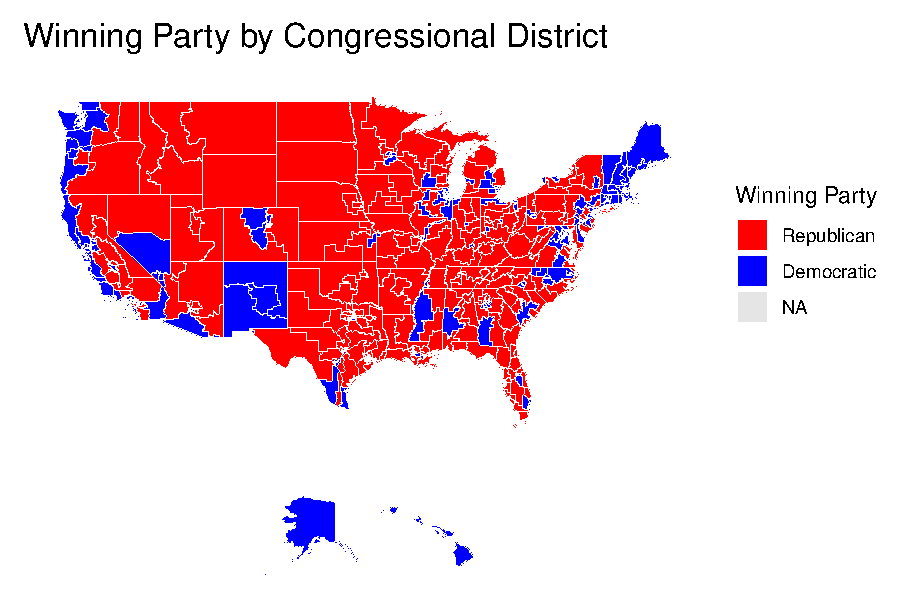
\includegraphics[width=0.9\textwidth]{plots/party_map.pdf}
\end{frame} 


\begin{frame}{Urban Index}
Our dependent variable of interest is the Urban Index from FiveThirtyEight.
 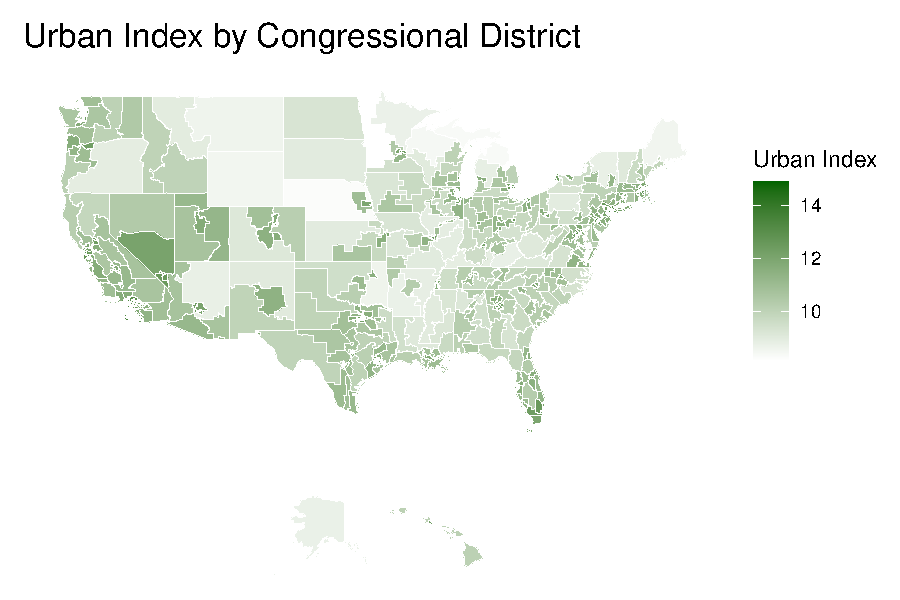
\includegraphics[width=0.9\textwidth]{plots/urbanindexmap.pdf}
\end{frame} 



\begin{frame}{Densities}
    \centering
    % First row
    \begin{minipage}{0.3\textwidth}
        \centering
        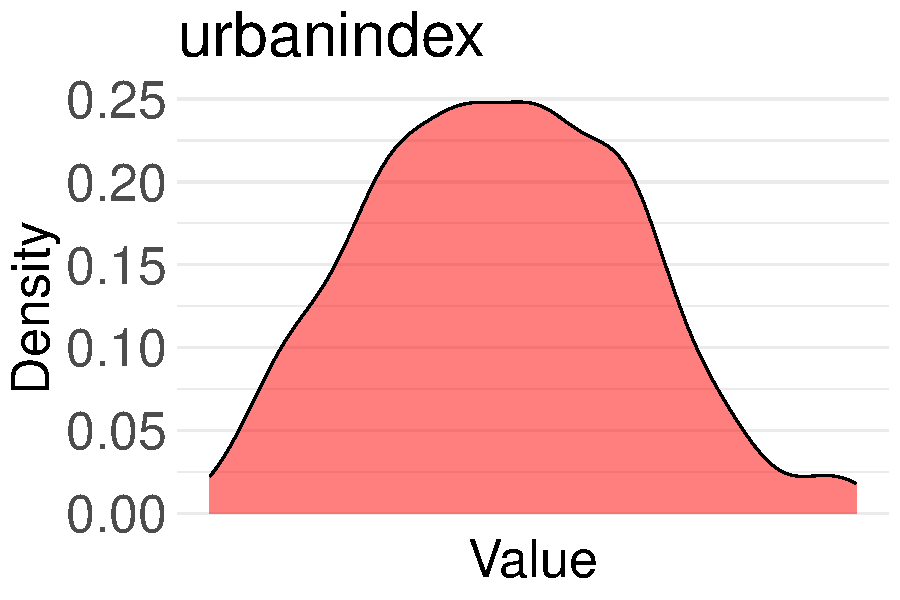
\includegraphics[width=\textwidth]{plots/urbanindex_density_plot.pdf}
    \end{minipage}
    \hfill
    \begin{minipage}{0.3\textwidth}
        \centering
        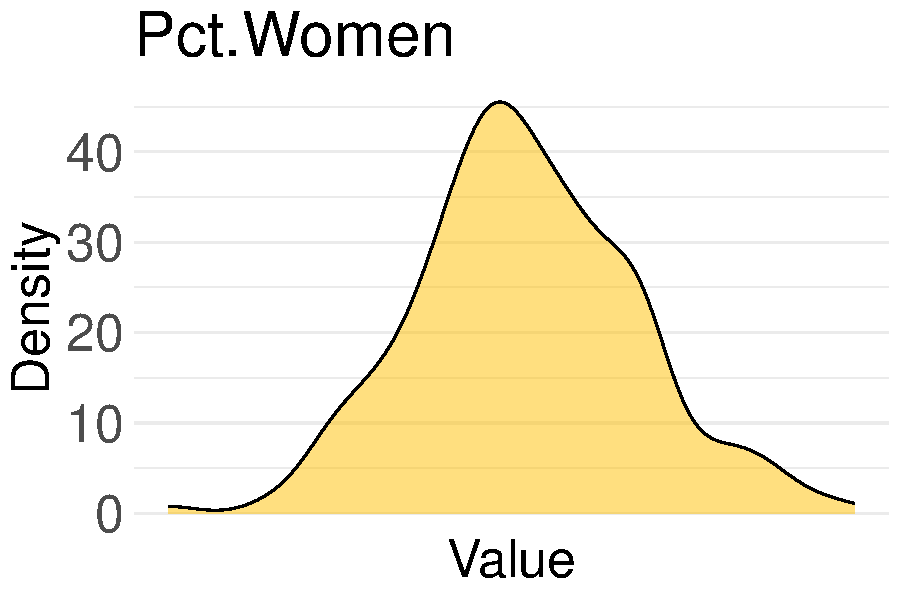
\includegraphics[width=\textwidth]{plots/Pct.Women_density_plot.pdf}
    \end{minipage}
    \hfill
    \begin{minipage}{0.3\textwidth}
        \centering
        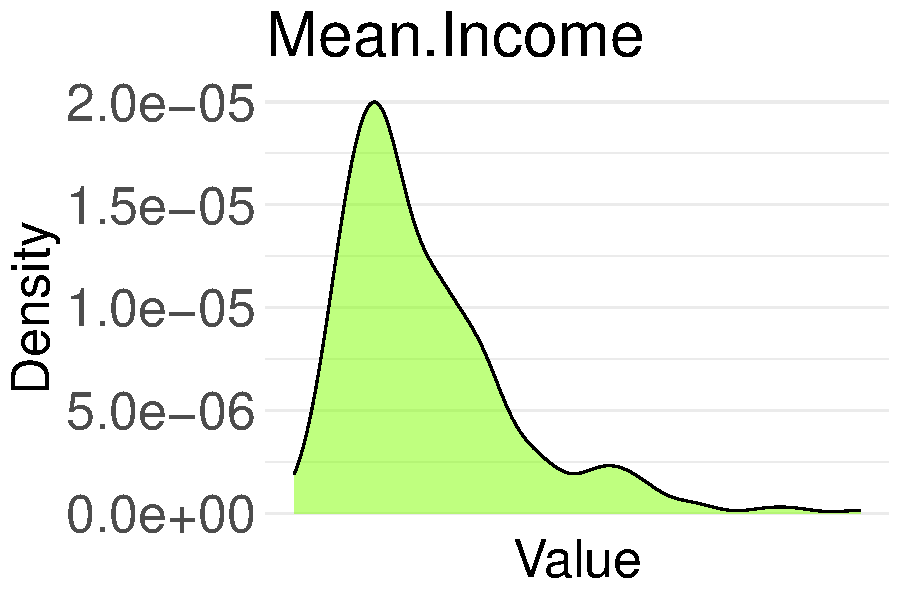
\includegraphics[width=\textwidth]{plots/Mean.Income_density_plot.pdf}
    \end{minipage}
    
    \vspace{0.2cm} % Add vertical space between rows

    % Second row
    \begin{minipage}{0.3\textwidth}
        \centering
        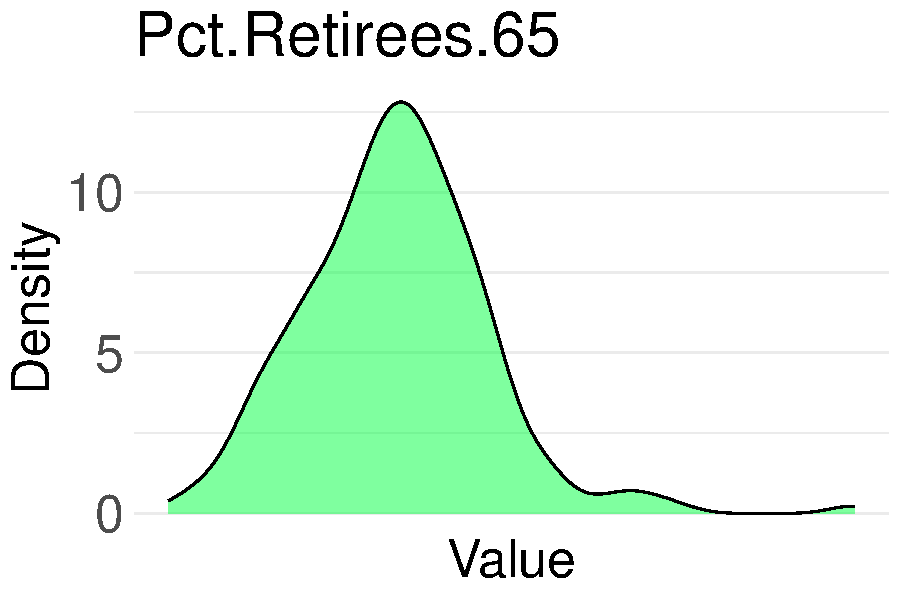
\includegraphics[width=\textwidth]{plots/Pct.Retirees.65_density_plot.pdf}
    \end{minipage}
    \hfill
    \begin{minipage}{0.3\textwidth}
        \centering
        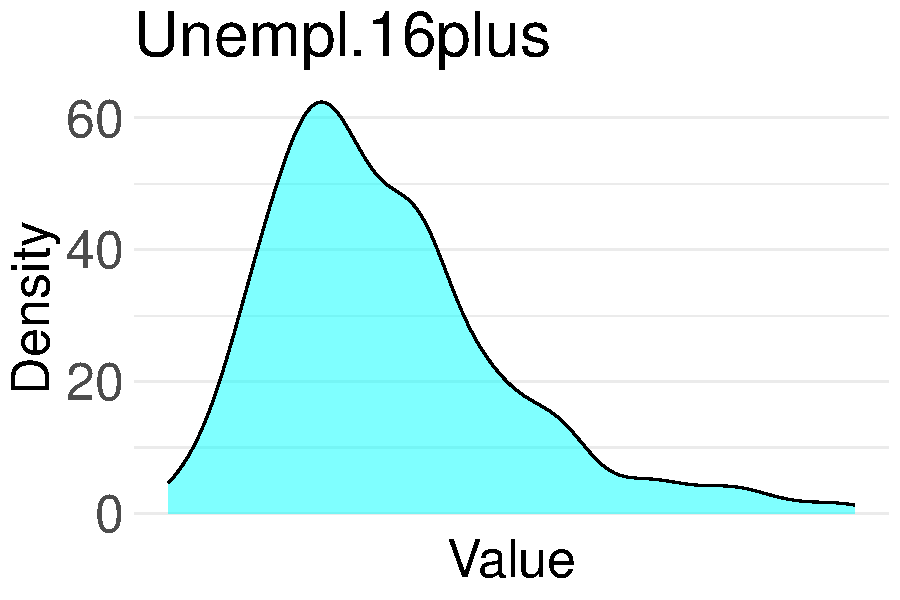
\includegraphics[width=\textwidth]{plots/Unempl.16plus_density_plot.pdf}
    \end{minipage}
    \hfill
    \begin{minipage}{0.3\textwidth}
        \centering
        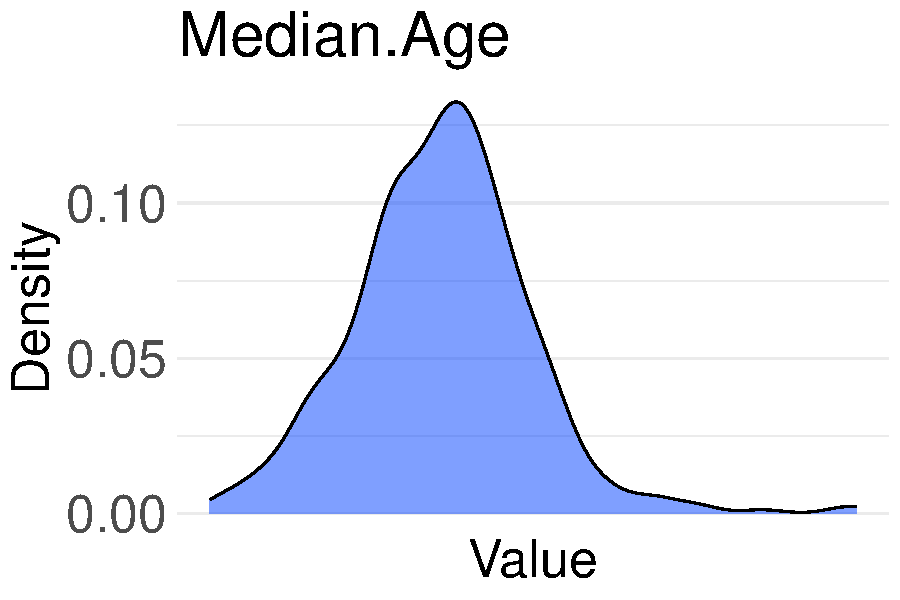
\includegraphics[width=\textwidth]{plots/Median.Age_density_plot.pdf}
    \end{minipage}
    
    \vspace{0.2cm} % Add vertical space between rows

    % Third row
    \begin{minipage}{0.3\textwidth}
        \centering
        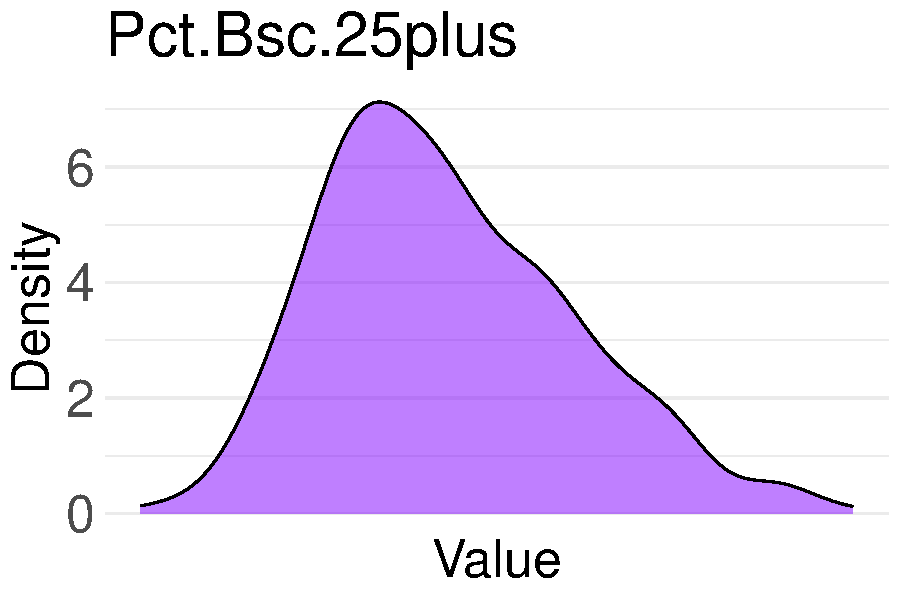
\includegraphics[width=\textwidth]{plots/Pct.Bsc.25plus_density_plot.pdf}
    \end{minipage}
    \hfill
    \begin{minipage}{0.3\textwidth}
        \centering
        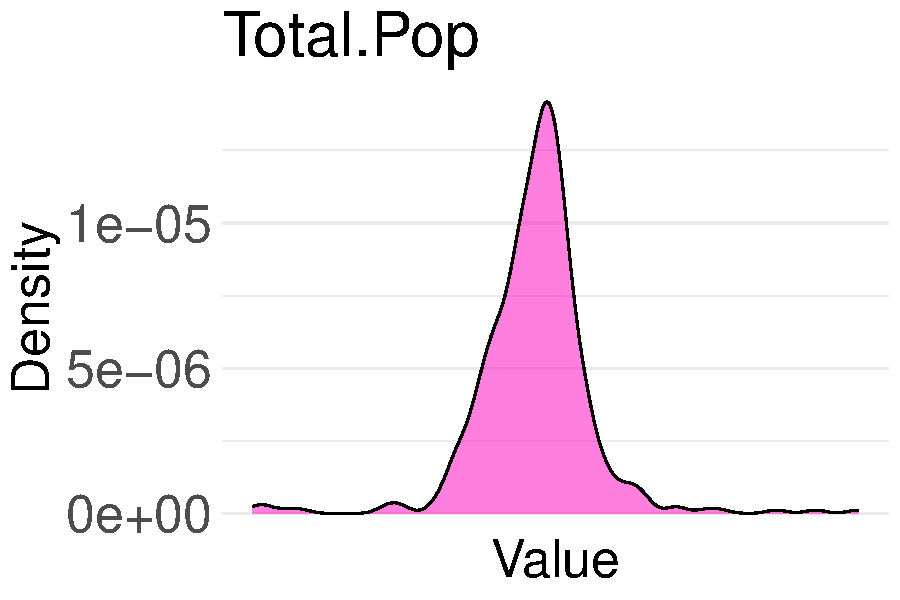
\includegraphics[width=\textwidth]{plots/Total.Pop_density_plot.pdf}
    \end{minipage} 
    \hfill
    \begin{minipage}{0.3\textwidth}
        \hfill
    \end{minipage}
\end{frame}


\begin{frame}{Correlation Matrix}
    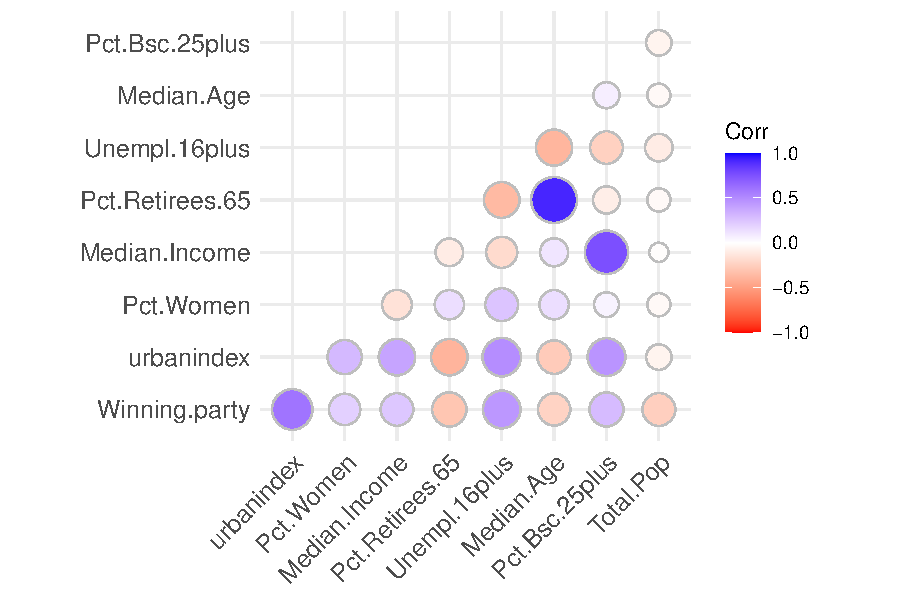
\includegraphics[width=0.9\textwidth]{plots/corrplot.pdf}
\end{frame}
%slide
% \begin{frame}
% \frametitle{Frame name}

\begin{frame}{Motivation for Hierarchical Modelling}
    \begin{figure}
    \centering
    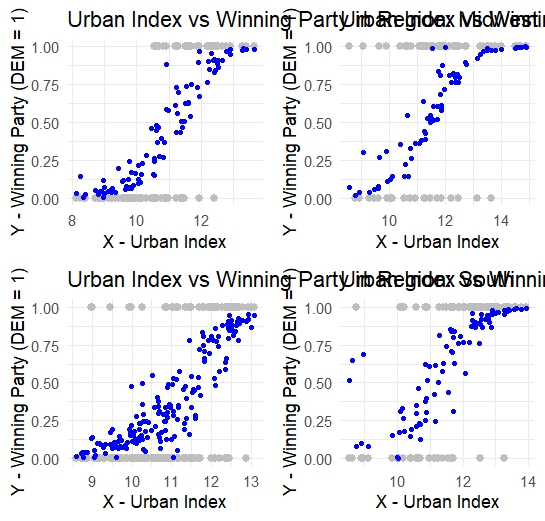
\includegraphics[width=0.95\textwidth]{plots/motivation_groupwise_scatterplot.jpeg} %%placeholder!!!!
    \caption{Your caption here}
\end{figure}

\end{frame}




% \begin{footnotesize}
% \begin{verbatim}
% # Set the maximum number of samples
% N <- 10000        
% # Pmf of x
% x <- 1        
% # Initialize a vector to store the final estimates
% estimates <- numeric(N)   
% # Write function to get estimate of the mean
% # for a given sample size 'n'

% get_est_mean <- function(lambda, n){
%   shelf <- numeric(n)    
%   for(i in 1:n){
%     x <- rpois(m, lambda[i])   #simulate i.i.d.
%                                 #Poisson for given lambda
%     shelf[i] <- mean(x)
%   }
%   return(mean(shelf))
% }

% \end{verbatim}
% \end{footnotesize}

% \end{frame}

\section{Model Setup}
%slide
\begin{frame}
  \frametitle{Model Assumptions}
  There are many people trying to predict US election outcomes, from the wealth of data available about voters. However we wanted to look at the voters in relation to their geography. In order to do this we assumed 
  \begin{itemize}
    \item District voting outcomes can be modeled via logistic regression 
    \item Districts are exchangable within each state and each state is exchangable within its region
    % would be nice to have a graphic showing the geographic hierachry 
    \item ??? 
  \end{itemize}
  \end{frame}

%slide
\begin{frame}
\frametitle{Model}
Let the response variable 'Winning Party' be \(y\), the predictor of interest 'Urban index' be \(x\), and the other covariates be a 15-dimensional vector \(z\). Let \(i\), \(j\), and \(k\) be the indices for the district, region, and state respectively. 

\[y_{i, j} \sim Ber.(logit^{-1}(\theta_{j}))\]

\[\theta_j := \beta_0, j + x_{i,j} * \beta_{1,j}  + z_{i, j}^T * \gamma_{1,j}\]

\[\beta_{1,j} \sim Gam.(1, \tau)\]

\[\tau \sim Normal(0, 1) \]  %placeholder!!!!


\end{frame}
\section{Priors}

%slide - prior place holder 
\begin{frame}
  \frametitle{Factor name}
  % what is it & reasoning

  % prior distribution equation 
  % \begin{center}
  %   \includegraphics[width=0.5\textwidth]{}
  % \end{center}

  % equation 
\end{frame}

%slide 
\begin{frame}
  \frametitle{Urbanization Index}
  % Script 
  Urbanization Index is a measure created by fivethirtyeight calculated based on populatin density of a given district.
  We assume that urbaniation has some positive impact on the likelihood of voting democrat, because urban areas tend to lean more democratic [source]. 
  However, we assume a regional effect as this relationship is likely more pronounced in more rural regions generally. % should we have a source here? 
  %prior distribution graph 
  \begin{center}
    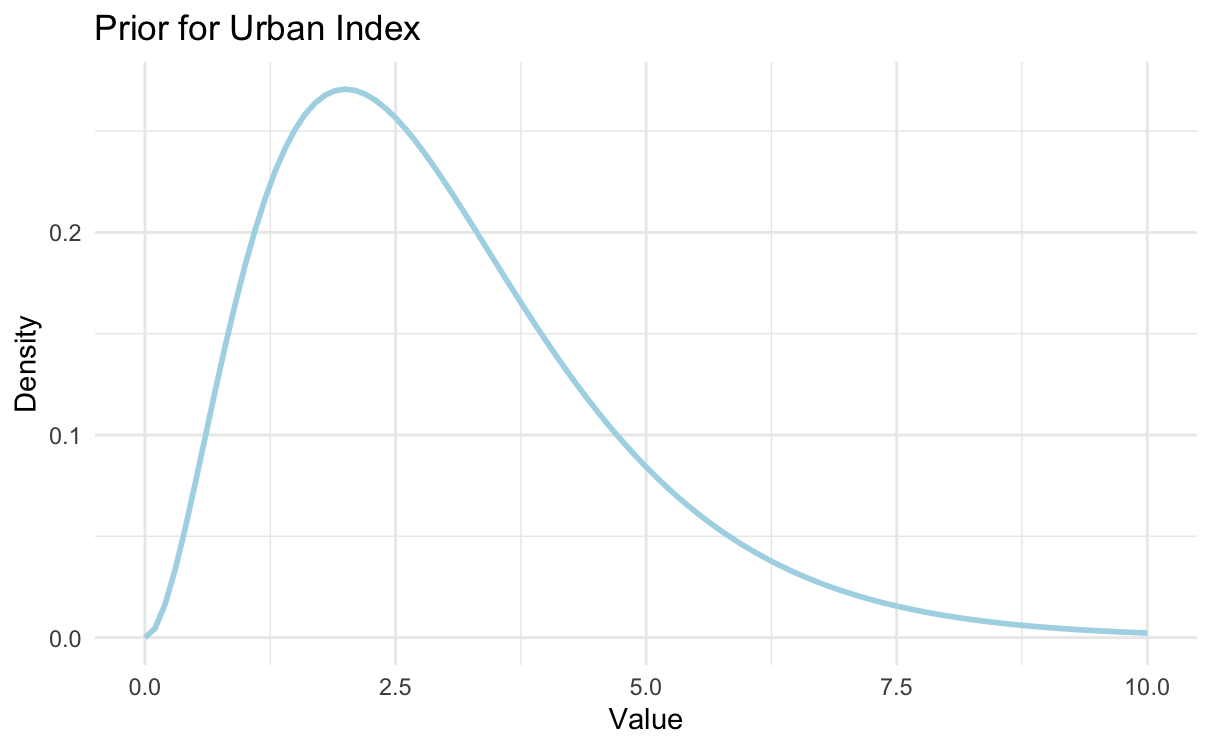
\includegraphics[width=0.5\textwidth]{plots/prior_urban.index.png}
  \end{center}
 
  
  % prior distribution equation 
  $$ \beta_{urbanindex} \sim Gamma(\alpha = 3, \beta = 1 )$$ 
  % explaination 
  \end{frame}

\begin{frame}
  \frametitle{Urbanization Category}
  % what is it - need to rethink 
  Urbanization category is the measure created by fivethirtyeight that bounds the numerical values of urban index into several buckets. 
  We assume that each of these categories with have a postive association 
  % prior distribution equation 

  % explaination 
\end{frame}

%slide 
\begin{frame}
  \frametitle{Total Population}
  % what is it 
  Since each district is drawn to have roughly the same population within each state, we think that this covariate will have a very small influence as there should be nearly no variance within a state. However, this effect maybe be state dependent. 
  % prior distribution equation 
  \begin{center}
    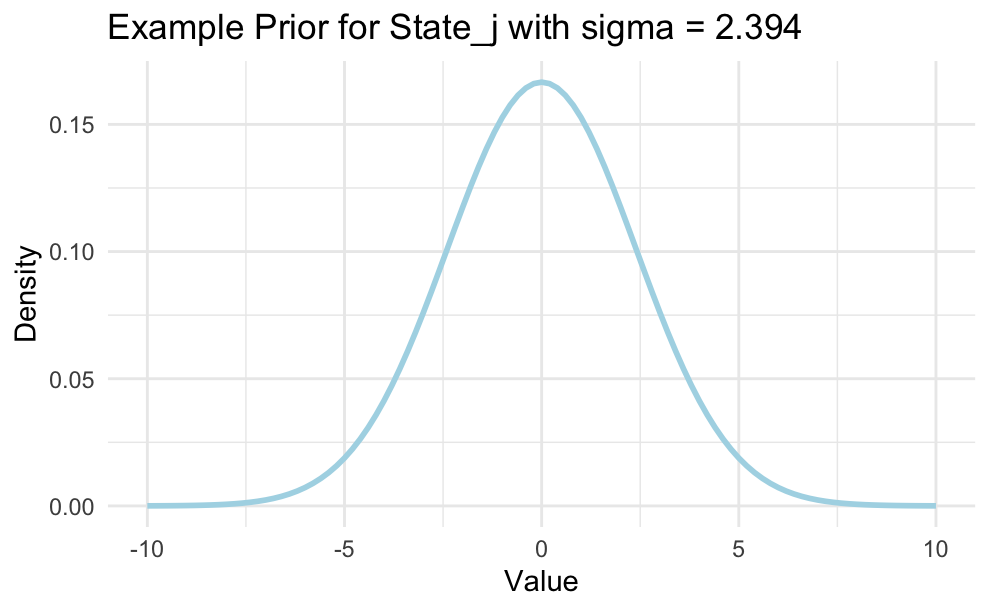
\includegraphics[width=0.5\textwidth]{plots/prior_total_pop.png}
  \end{center}
  
  % explaination 
  $$ \beta_{total.pop} | state \sim  N(0, \sigma_{state})$$
\end{frame}

%slide 
\begin{frame}
  \frametitle{Percentage Women}
  % what is it 
  We found that women tend to lean more democratic and have higher turnout than men. Leading us to believe there should be a positive association between percentage women in a district and probability of voting democratic. 
  However percentage of women isn't a variable that varies greatly with geography so we assume if there is an effect that it will be quite small.  
  % prior distribution equation 
  \begin{center}
    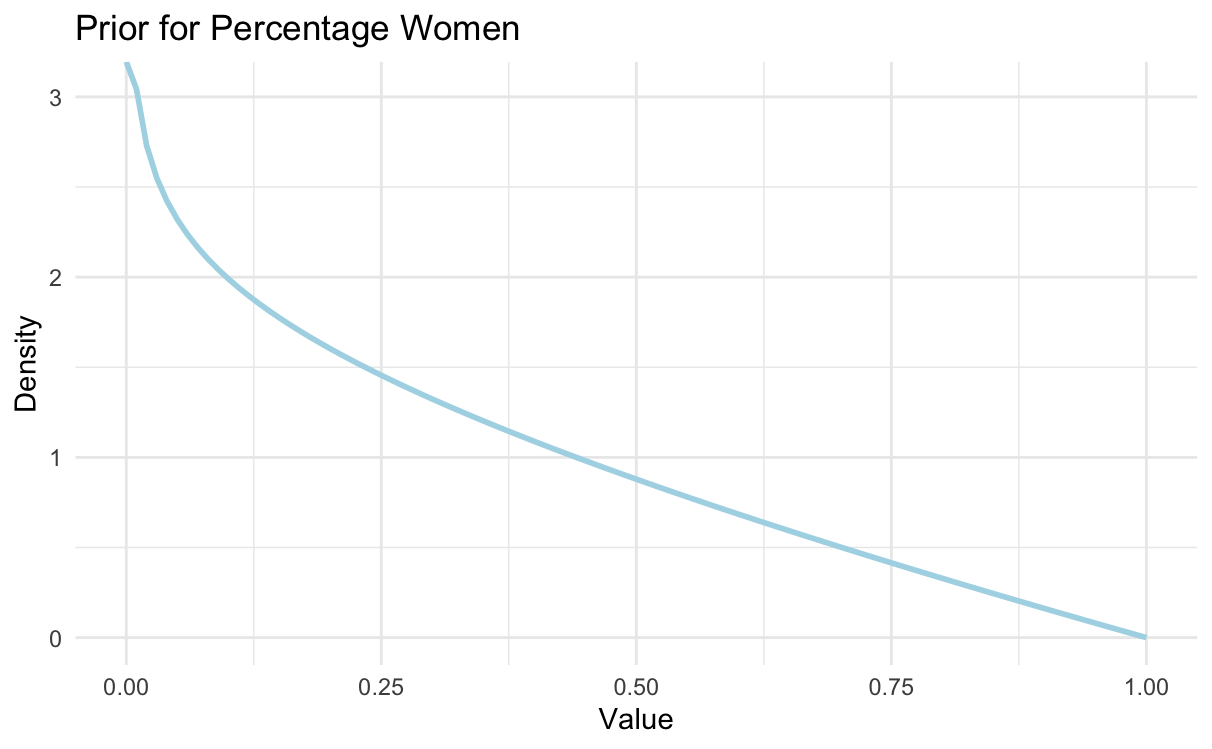
\includegraphics[width=0.5\textwidth]{plots/prior_pct.women.png}
  \end{center}
  
  % explaination 
  $$ \beta_{pct.women} \sim Beta(\alpha = \frac{6}{7}, \beta = 2) $$
\end{frame}

\begin{frame}
  \frametitle{Percentage of Population over 25 with Bachelors Degree}
  % what is it & reasoning
  We found that those holding a bachelors degree or higher education lean democratic however they make up a small part of the population 
  % prior distribution equation 
  \begin{center}
    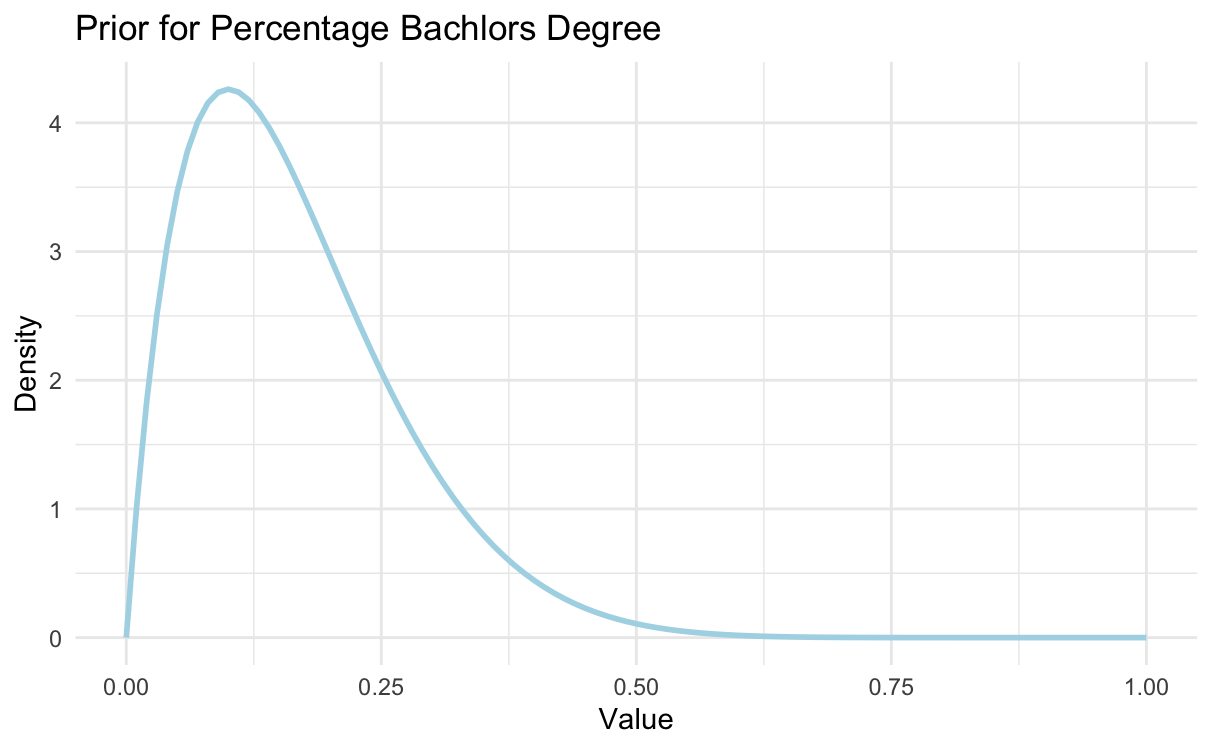
\includegraphics[width=0.9\textwidth]{plots/prior_pct.bachelors.png}
  \end{center}
  

  % equation 
  $$  \beta_{pct.bachelors} \sim Beta( \alpha = 1 , \beta = 10 )$$
\end{frame}



\section{Pooled Model}

%slide
\begin{frame}
\frametitle{Pooled Model - Description}

The simplest type of model where no hierarchies are taken into account:

\[y_{i, j} \sim Ber.(logit^{-1}(\theta))\]

\[\theta := \beta_0 + x_{i} * \beta_{1}  + z_{i}^T * \gamma_{1}\]

\[\beta_{1,j} \sim Gam.(3, 1)\]

\end{frame}

\begin{frame}{Pooled Model - Trace Plot}

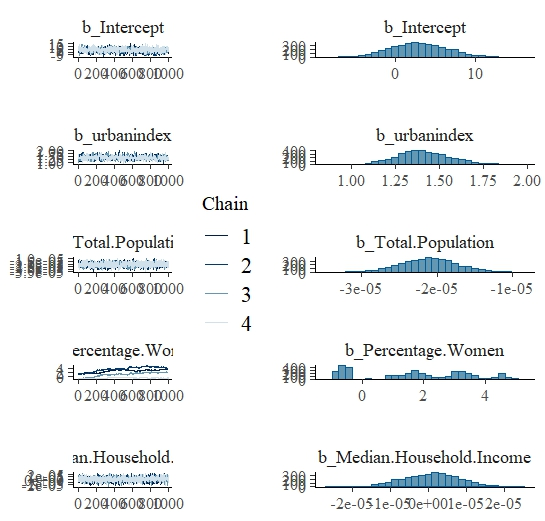
\includegraphics[width=0.9\textwidth]{plots/chains_pooled_model_default_priors_1.jpeg}

\end{frame}

\begin{frame}{Pooled Model - Trace Plot 2}

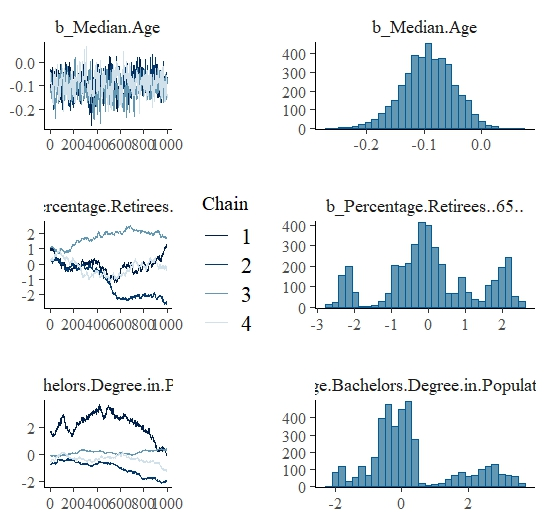
\includegraphics[width=0.9\textwidth]{plots/chains_pooled_model_default_priors_2.jpeg}

    
\end{frame}


\section{Unpooled Model}

%slide
\begin{frame}
\frametitle{Description - Unpooled Model}

\end{frame}

\section{Results - Hierarchical Model}

%slide
\begin{frame}
\frametitle{Varying Intercept Model}

\begin{center}
    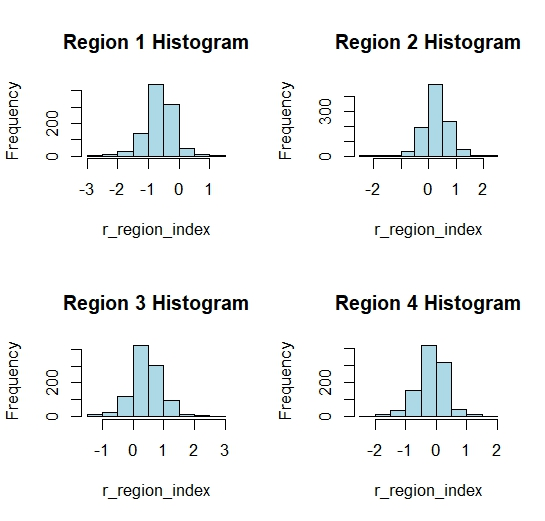
\includegraphics[width=0.8\textwidth]{placeholder_hist_varying_intercept_1_level.jpeg}
\end{center}

\end{frame}


\begin{frame}
  \frametitle{Varying Intercept Model - II}%% wasn't rendering properly 
  
  % \begin{table} \centering
  %   \caption{Descriptive Statistics by Region} 
  %   \label{table:stats}
  %   \resizebox{\textwidth}{!}{ % Resizing the table to fit the frame width
  %   \begin{tabular}{@{\extracolsep{5pt}} cccccccccccc} 
  %   \toprule
  %   & Region & Variable & Mean & Median & SD & MAD & Q5 & Q95 & Rhat & ESS\_Bulk & ESS\_Tail \\ 
  %   \midrule
  %   1 & $1$ & r\_region\_index & $-0.661$ & $-0.627$ & $0.486$ & $0.405$ & $-1.484$ & $0.023$ & $1.014$ & $221.604$ & $240.881$ \\ 
  %   2 & $2$ & r\_region\_index & $0.272$ & $0.273$ & $0.496$ & $0.388$ & $-0.443$ & $1.035$ & $1.010$ & $249.762$ & $277.608$ \\ 
  %   3 & $3$ & r\_region\_index & $0.424$ & $0.410$ & $0.513$ & $0.417$ & $-0.414$ & $1.242$ & $1.004$ & $267.517$ & $238.103$ \\ 
  %   4 & $4$ & r\_region\_index & $-0.164$ & $-0.138$ & $0.495$ & $0.419$ & $-1.008$ & $0.534$ & $1.014$ & $262.794$ & $271.583$ \\ 
  %   \bottomrule
  %   \end{tabular}
  %   } % End of resizebox
  % \end{table}
\end{frame}



\section{Results - Varying Intercept Model}

%slide
\begin{frame}
\frametitle{=----}

\end{frame}

\section{Centred vs Non-centred Parameterisation/ Sampling Investigation with STAN}

%slide
\begin{frame}
\frametitle{STAN Code}

\end{frame}

\section{Raw References}

\begin{frame}{Raw references}
    \begin{itemize}
        \item stargazer
        \item tidybayes
        \item brms, stan
    \end{itemize}
\end{frame}




\end{document}
